\documentclass[12pt,oneside]{amsart}

\title{Math 287 Homework 10}
\author{Andrew Moore}
\date{November 28, 2021} % the due date of the homework

\usepackage[T1]{fontenc}
\usepackage{amsmath,amsfonts,amssymb,amsthm}
\usepackage[letterpaper,margin=1.5in]{geometry}
\usepackage{fancyhdr}
\usepackage{tikz}
\pagestyle{fancy}
\usepackage{enumitem}

% Extra space between lines
\linespread{2.4}

\theoremstyle{remark}
\newtheorem{exer}{Exercise}
\newtheorem{claim}{Claim}[exer]

\newcommand{\bfN}{\mathbf{N}}
\newcommand{\bfZ}{\mathbf{Z}}


\newenvironment{answer}{\bigskip\noindent\emph{Answer.}}{\hfill$\diamond$\newline}

\begin{document}
\maketitle

\begin{exer}
Suppose $f$ is a function $f : \{a,b,c\} \to \{u,v\}$ and we have $f(a)=u$ and $f(b)=u$.
How should we define $f(c)$ if we want $f$ to be surjective (onto)?
\end{exer}

\begin{answer}
We should define $f(c)=v$.
Then $f$ is given by the table:
\[
\linespread{1.2}\selectfont % This is only needed because of \linespread{2.4} that is used for homework
\begin{array}{c|rrr}
x & a & b & c \\
\hline
f(x) & u & u & v \\
\end{array}
\]

% The linespread{2.4} would make the table way too spaced out. So we temporarily turn it off. The linspread change only affects within the \[ ... \]. After this display math ends, we’ll be back to linespread{2.4}. If you type arrays or tables in documents that don’t have linespread changes, then you can leave out the \linespread{1.2}\selectfont line.

% LaTeX: The {c|rrr} makes our table have 4 columns. The first column will be center-aligned, there will be a vertical separater line, and then the next three columns will be right-aligned.

We can represent $f$ pictorially by:
\begin{center}
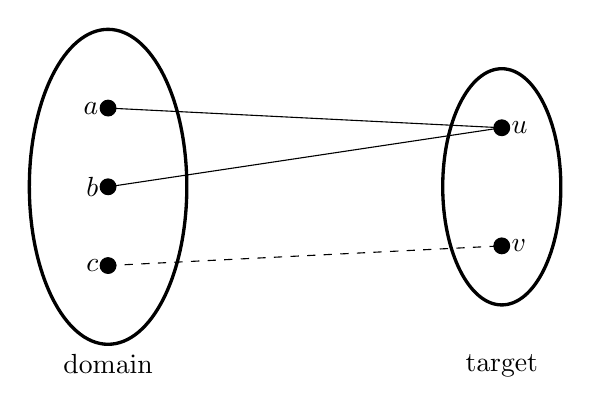
\begin{tikzpicture}

  \draw[very thick] (0,0) ellipse[x radius=1, y radius=2];
  \node[below] at (0,-2) {domain};

  \draw[very thick] (5,0) ellipse[x radius=0.75, y radius=1.5];
  \node[below] at (5,-2) {target};

  \filldraw[black,fill=black] (0,1) circle[radius=0.1] node[left] {$a$};
  \filldraw[black,fill=black] (0,0) circle[radius=0.1] node[left] {$b$};
  \filldraw[black,fill=black] (0,-1) circle[radius=0.1] node[left] {$c$};

  \filldraw[black,fill=black] (5,0.75) circle[radius=0.1] node[right] {$u$};
  \filldraw[black,fill=black] (5,-0.75) circle[radius=0.1] node[right] {$v$};

  \draw (0,1) -- (5,0.75);
  \draw (0,0) -- (5,0.75);
  \draw[dashed] (0,-1) -- (5,-0.75);

\end{tikzpicture}
\end{center}
We used a dashed line to show $f(c)=v$ that was the answer to the question.
\end{answer}

% LaTeX: There’s a lot going on here. The important parts are that \draw draws lines and other shaps, \filldraw draws them and also fills them in, common shapes like circle and ellipse can be said directly, and for line segments we can use -- to connect a start point to an end point. Also node creates points where we can add label text.

\newpage
\begin{exer}
% Now modify the table and tikzpicture to answer this question:
Suppose $f$ is a function $f: \{a, b, c\} \to \{u, v, w\}$  and we have $f(a) = u, f(b) = w$. How should we define $f(c)$ if we want $f$ to be injective (one-to-one)?
% Once you understand the question and know how to answer it, copy and modify the table and the graphic from the first question. Answer this question on a new page (after the first question).
\end{exer}

\begin{answer}
We should define $f(c) = v$.

Then $f$ is given by the table:
\[
\linespread{1.2}\selectfont % This is only needed because of \linespread{2.4} that is used for homework
\begin{array}{c|rrr}
x & a & b & c \\
\hline
f(x) & u & w & v \\
\end{array}
\]

We can represent $f$ pictorially by:
\begin{center}
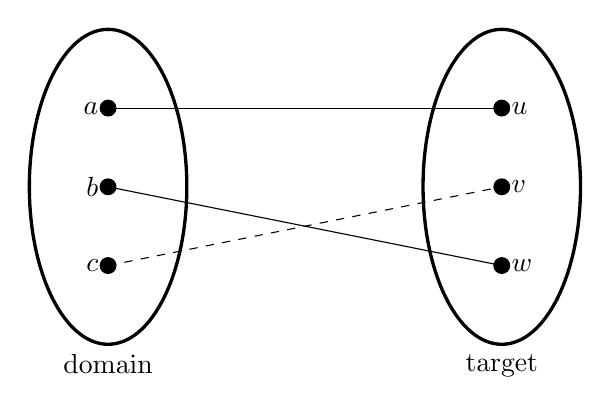
\begin{tikzpicture}

  \draw[very thick] (0,0) ellipse[x radius=1, y radius=2];
  \node[below] at (0,-2) {domain};

  \draw[very thick] (5,0) ellipse[x radius=1, y radius=2];
  \node[below] at (5,-2) {target};

  \filldraw[black,fill=black] (0,1) circle[radius=0.1] node[left] {$a$};
  \filldraw[black,fill=black] (0,0) circle[radius=0.1] node[left] {$b$};
  \filldraw[black,fill=black] (0,-1) circle[radius=0.1] node[left] {$c$};

  \filldraw[black,fill=black] (5,1) circle[radius=0.1] node[right] {$u$};
  \filldraw[black,fill=black] (5,0) circle[radius=0.1] node[right] {$v$};
  \filldraw[black,fill=black] (5,-1) circle[radius=0.1] node[right] {$w$};

  \draw (0,1) -- (5,1);
  \draw (0,0) -- (5,-1);
  \draw[dashed] (0,-1) -- (5,0);

\end{tikzpicture}
\end{center}
We used a dashed line to show $f(c)=v$ that was the answer to the question.
\end{answer}

\newpage
\begin{exer}
Finally, redo one problem from a previous homework assignment. Your score will count for this homework, not the previous one. Along with your answer, write a short reflection essay (1-2 paragraphs) about what you learned.
\end{exer}

\end{document}
